%------------------------------------------------------------------------------%
\section{Implementación de la propuesta}
%------------------------------------------------------------------------------%

\subsection{Planificación y estimación}

\begin{table}
	\small\centering
    \caption{Cronograma y planificación de los \textit{sprints}. La ``S'' es de \textit{sprint}.}
    \label{tab:sprints}
    \begin{NiceTabular}{p{4.5cm}|c|c|c|c|c|c|c|c|c|c|c|c|c}[
        code-before = 
        \cellcolor{mygreen}{2-2, 2-3, 2-8, 2-11}
        \cellcolor{mygreen}{3-2, 3-3, 3-8, 3-11}
        \rectanglecolor{mygreen}{4-4}{4-6}
        \rectanglecolor{mygreen}{5-4}{5-7}\rectanglecolor{mygreen}{5-9}{5-13}
        \cellcolor{mygreen}{6-8, 6-11}
        \rectanglecolor{mygreen}{7-4}{7-13}
        \rectanglecolor{mygreen}{8-7}{8-13}
        \cellcolor{mygreen}{9-7, 9-10, 9-13}
     ]
        \hline
        Actividad                  & S1& S2& S3& S4& S5& S6& S7& S8& S9&S10&S11&S12\\
        \hline
        Investigación del producto &   &   &   &   &   &   &   &   &   &   &   &   \\
        \hline
        Diseño                     &   &   &   &   &   &   &   &   &   &   &   &   \\
        \hline
        Desarrollo red neuronal    &   &   &   &   &   &   &   &   &   &   &   &   \\
        \hline
        Desarrollo aplicación web  &   &   &   &   &   &   &   &   &   &   &   &   \\
        \hline
        Retroalimentación          &   &   &   &   &   &   &   &   &   &   &   &   \\
        \hline
        Desarrollo 
        API             &   &   &   &   &   &   &   &   &   &   &   &   \\
        \hline
        Entrenamiento y mejora red neuronal &   &   &   &   &   &   &   &   &   &   &   \\
        \hline
        Lanzamiento PMV            &   &   &   &   &   &   &   &   &   &   &   &   \\
        \hline      
    \end{NiceTabular}
\end{table}



\begin{table}
    \small\centering
    \caption{Costos del proyecto.}
    \label{tab:costos}
    \begin{tabular}{p{4.5cm}rrrr}
        \toprule
        Recursos Humanos & Cantidad & Costo mensual & Meses & Subtotal \\
        \midrule
        \textit{Senior FullStack Developer} & 1 & 50,000 & 3 & 150,000 \\
        \textit{Junior Fullstack Developer} & 1 & 28,000 & 3 & 84,000 \\
        \textit{Senior Ux Design}er & 1 & 35,000 & 3 & 105,000 \\
        Arquitecto de sistemas \textit{Cloud mid level} & 1 & 75,000 & 3 & 225,000 \\
        \textit{Product Owner }& 1 & 65,000 & 3 & 195,000 \\
        \midrule
        &  &  &  Total & 759,000 \\
        \bottomrule
        \toprule
        Servicios & Cantidad & Costo mensual & Meses & Subtotal \\
        \midrule
        Servicios Azure & 1 & 51,413 & 3 & 154,240 \\
        \midrule
        &  &  &  Total & 154,240 \\
        \bottomrule
        \toprule 
        Materiales & & Cantidad & Costo & Subtotal \\
        \midrule
        \textit{Laptop hp zbook 14 Firefly G8} & & 4 & 35,000 & 140,000 \\
        \textit{Macbook Pro MKGP3E/A} & & 2 & 49,000 & 98,000 \\
        \midrule
        &  &  Total &  & 238,000 \\
        \bottomrule 
        \toprule 
        Infraestructura &  & Costo mensual & Meses & Subtotal \\
        \midrule
        Internet & & 3,000 & 14 & 42,000 \\
        \midrule
        &  &  Total &  & 42,000 \\
        \bottomrule
        \toprule 
        \multicolumn{4}{r}{\textbf{Total global del proyecto}} & \textbf{1,193,240} \\
        \bottomrule
    \end{tabular}
\end{table}

\subsection{Prototipo}

\begin{figure}
    \centering
    \caption[Diagrama del funcionamiento de la aplicación.]{Diagrama del funcionamiento de la aplicación.}
    \label{fig:funcionamiento}
    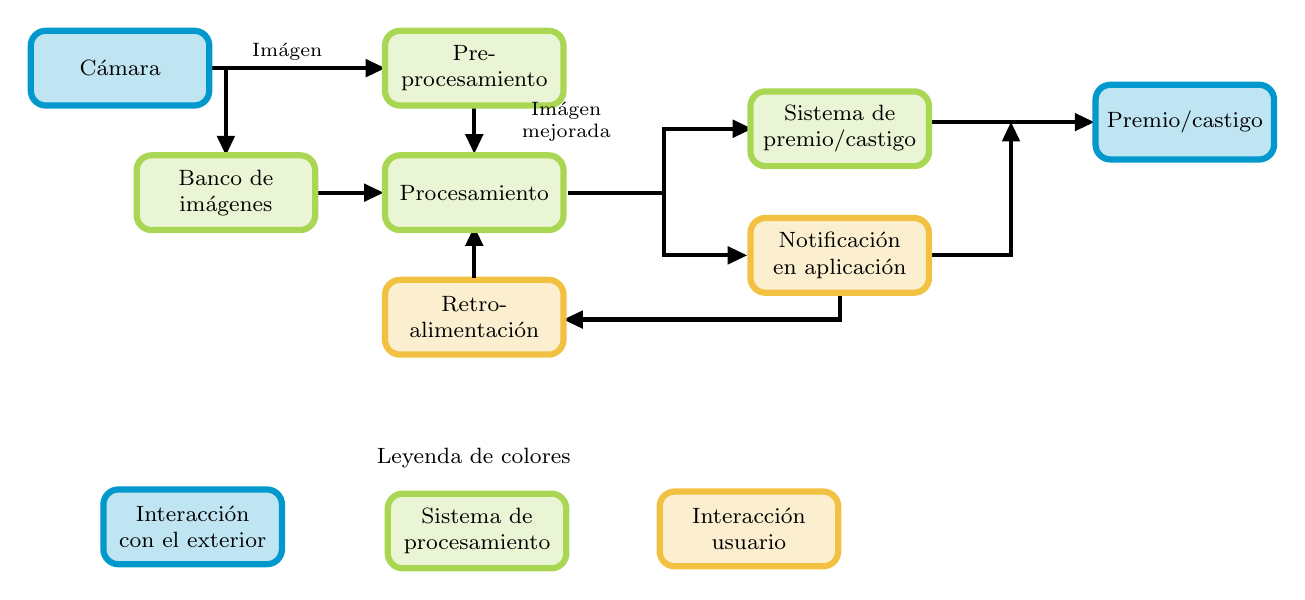
\begin{tikzpicture}[x=0.75pt,y=0.75pt,yscale=-1,xscale=1]
%uncomment if require: \path (0,480); %set diagram left start at 0, and has height of 480

%Straight Lines [id:da49883994500921447] 
\draw [line width=1.5]    (296.67,97.67) -- (343.07,97.67) -- (343.07,127.87) -- (379.07,127.87) ;
\draw [shift={(383.07,127.87)}, rotate = 180] [fill={rgb, 255:red, 0; green, 0; blue, 0 }  ][line width=0.08]  [draw opacity=0] (9.29,-4.46) -- (0,0) -- (9.29,4.46) -- cycle    ;
%Straight Lines [id:da2905724578829102] 
\draw [line width=1.5]    (296.67,97.67) -- (343.07,97.67) -- (343.07,66.87) -- (381.47,66.87) ;
\draw [shift={(385.47,66.87)}, rotate = 180] [fill={rgb, 255:red, 0; green, 0; blue, 0 }  ][line width=0.08]  [draw opacity=0] (9.29,-4.46) -- (0,0) -- (9.29,4.46) -- cycle    ;
%Straight Lines [id:da10483512115459537] 
\draw [line width=1.5]    (124.67,37.67) -- (204.67,37.67) ;
\draw [shift={(208.67,37.67)}, rotate = 180] [fill={rgb, 255:red, 0; green, 0; blue, 0 }  ][line width=0.08]  [draw opacity=0] (9.29,-4.46) -- (0,0) -- (9.29,4.46) -- cycle    ;
%Straight Lines [id:da4860403173310909] 
\draw [line width=1.5]    (175.87,97.67) -- (203.87,97.67) ;
\draw [shift={(207.87,97.67)}, rotate = 180] [fill={rgb, 255:red, 0; green, 0; blue, 0 }  ][line width=0.08]  [draw opacity=0] (9.29,-4.46) -- (0,0) -- (9.29,4.46) -- cycle    ;
%Straight Lines [id:da39629635865875956] 
\draw [line width=1.5]    (469.47,63.67) -- (546.27,63.67) ;
\draw [shift={(550.27,63.67)}, rotate = 180] [fill={rgb, 255:red, 0; green, 0; blue, 0 }  ][line width=0.08]  [draw opacity=0] (9.29,-4.46) -- (0,0) -- (9.29,4.46) -- cycle    ;
%Straight Lines [id:da6360560713651083] 
\draw [line width=1.5]    (343.07,66.87) -- (385.47,66.87) ;
%Straight Lines [id:da7217883827854481] 
\draw [line width=1.5]    (470.27,127.87) -- (510.27,127.87) -- (510.27,67.67) ;
\draw [shift={(510.27,63.67)}, rotate = 90] [fill={rgb, 255:red, 0; green, 0; blue, 0 }  ][line width=0.08]  [draw opacity=0] (9.29,-4.46) -- (0,0) -- (9.29,4.46) -- cycle    ;
%Straight Lines [id:da9212509405858289] 
\draw [line width=1.5]    (427.74,145.47) -- (427.74,158.8) -- (298.67,158.8) ;
\draw [shift={(294.67,158.8)}, rotate = 360] [fill={rgb, 255:red, 0; green, 0; blue, 0 }  ][line width=0.08]  [draw opacity=0] (9.29,-4.46) -- (0,0) -- (9.29,4.46) -- cycle    ;
%Straight Lines [id:da7493384106097625] 
\draw [line width=1.5]    (132,38.8) -- (132,75.6) ;
\draw [shift={(132,79.6)}, rotate = 270] [fill={rgb, 255:red, 0; green, 0; blue, 0 }  ][line width=0.08]  [draw opacity=0] (9.29,-4.46) -- (0,0) -- (9.29,4.46) -- cycle    ;
%Rounded Rect [id:dp5515000815065423] 
\draw  [color={rgb, 255:red, 0; green, 152; blue, 205 }  ,draw opacity=1 ][fill={rgb, 255:red, 0; green, 152; blue, 205 }  ,fill opacity=0.25 ][line width=2.25]  (38,26.87) .. controls (38,22.89) and (41.22,19.67) .. (45.2,19.67) -- (116.8,19.67) .. controls (120.78,19.67) and (124,22.89) .. (124,26.87) -- (124,48.47) .. controls (124,52.44) and (120.78,55.67) .. (116.8,55.67) -- (45.2,55.67) .. controls (41.22,55.67) and (38,52.44) .. (38,48.47) -- cycle ;
%Rounded Rect [id:dp32085170046138056] 
\draw  [color={rgb, 255:red, 0; green, 152; blue, 205 }  ,draw opacity=1 ][fill={rgb, 255:red, 0; green, 152; blue, 205 }  ,fill opacity=0.25 ][line width=2.25]  (73,247.87) .. controls (73,243.89) and (76.22,240.67) .. (80.2,240.67) -- (151.8,240.67) .. controls (155.78,240.67) and (159,243.89) .. (159,247.87) -- (159,269.47) .. controls (159,273.44) and (155.78,276.67) .. (151.8,276.67) -- (80.2,276.67) .. controls (76.22,276.67) and (73,273.44) .. (73,269.47) -- cycle ;
%Rounded Rect [id:dp20895200609973108] 
\draw  [color={rgb, 255:red, 0; green, 152; blue, 205 }  ,draw opacity=1 ][fill={rgb, 255:red, 0; green, 152; blue, 205 }  ,fill opacity=0.25 ][line width=2.25]  (551,52.87) .. controls (551,48.89) and (554.22,45.67) .. (558.2,45.67) -- (629.8,45.67) .. controls (633.78,45.67) and (637,48.89) .. (637,52.87) -- (637,74.47) .. controls (637,78.44) and (633.78,81.67) .. (629.8,81.67) -- (558.2,81.67) .. controls (554.22,81.67) and (551,78.44) .. (551,74.47) -- cycle ;
%Rounded Rect [id:dp8032697712302126] 
\draw  [color={rgb, 255:red, 169; green, 215; blue, 83 }  ,draw opacity=1 ][fill={rgb, 255:red, 169; green, 215; blue, 83 }  ,fill opacity=0.25 ][line width=2.25]  (210,249.87) .. controls (210,245.89) and (213.22,242.67) .. (217.2,242.67) -- (288.8,242.67) .. controls (292.78,242.67) and (296,245.89) .. (296,249.87) -- (296,271.47) .. controls (296,275.44) and (292.78,278.67) .. (288.8,278.67) -- (217.2,278.67) .. controls (213.22,278.67) and (210,275.44) .. (210,271.47) -- cycle ;
%Rounded Rect [id:dp33703696522885096] 
\draw  [color={rgb, 255:red, 169; green, 215; blue, 83 }  ,draw opacity=1 ][fill={rgb, 255:red, 169; green, 215; blue, 83 }  ,fill opacity=0.25 ][line width=2.25]  (89,86.87) .. controls (89,82.89) and (92.22,79.67) .. (96.2,79.67) -- (167.8,79.67) .. controls (171.78,79.67) and (175,82.89) .. (175,86.87) -- (175,108.47) .. controls (175,112.44) and (171.78,115.67) .. (167.8,115.67) -- (96.2,115.67) .. controls (92.22,115.67) and (89,112.44) .. (89,108.47) -- cycle ;
%Rounded Rect [id:dp23380782720527082] 
\draw  [color={rgb, 255:red, 242; green, 193; blue, 65 }  ,draw opacity=1 ][fill={rgb, 255:red, 242; green, 193; blue, 65 }  ,fill opacity=0.25 ][line width=2.25]  (341,248.87) .. controls (341,244.89) and (344.22,241.67) .. (348.2,241.67) -- (419.8,241.67) .. controls (423.78,241.67) and (427,244.89) .. (427,248.87) -- (427,270.47) .. controls (427,274.44) and (423.78,277.67) .. (419.8,277.67) -- (348.2,277.67) .. controls (344.22,277.67) and (341,274.44) .. (341,270.47) -- cycle ;
%Rounded Rect [id:dp6654468042418796] 
\draw  [color={rgb, 255:red, 242; green, 193; blue, 65 }  ,draw opacity=1 ][fill={rgb, 255:red, 242; green, 193; blue, 65 }  ,fill opacity=0.25 ][line width=2.25]  (208.67,146.87) .. controls (208.67,142.89) and (211.89,139.67) .. (215.87,139.67) -- (287.47,139.67) .. controls (291.45,139.67) and (294.67,142.89) .. (294.67,146.87) -- (294.67,168.47) .. controls (294.67,172.44) and (291.45,175.67) .. (287.47,175.67) -- (215.87,175.67) .. controls (211.89,175.67) and (208.67,172.44) .. (208.67,168.47) -- cycle ;
%Rounded Rect [id:dp08221832448986155] 
\draw  [color={rgb, 255:red, 169; green, 215; blue, 83 }  ,draw opacity=1 ][fill={rgb, 255:red, 169; green, 215; blue, 83 }  ,fill opacity=0.25 ][line width=2.25]  (384.74,56.07) .. controls (384.74,52.09) and (387.96,48.87) .. (391.94,48.87) -- (463.54,48.87) .. controls (467.52,48.87) and (470.74,52.09) .. (470.74,56.07) -- (470.74,77.67) .. controls (470.74,81.64) and (467.52,84.87) .. (463.54,84.87) -- (391.94,84.87) .. controls (387.96,84.87) and (384.74,81.64) .. (384.74,77.67) -- cycle ;
%Rounded Rect [id:dp5392340882455937] 
\draw  [color={rgb, 255:red, 242; green, 193; blue, 65 }  ,draw opacity=1 ][fill={rgb, 255:red, 242; green, 193; blue, 65 }  ,fill opacity=0.25 ][line width=2.25]  (384.74,117.07) .. controls (384.74,113.09) and (387.96,109.87) .. (391.94,109.87) -- (463.54,109.87) .. controls (467.52,109.87) and (470.74,113.09) .. (470.74,117.07) -- (470.74,138.67) .. controls (470.74,142.64) and (467.52,145.87) .. (463.54,145.87) -- (391.94,145.87) .. controls (387.96,145.87) and (384.74,142.64) .. (384.74,138.67) -- cycle ;
%Straight Lines [id:da3463881313946451] 
\draw [line width=1.5]    (251.67,56.87) -- (251.67,74.8) ;
\draw [shift={(251.67,78.8)}, rotate = 270] [fill={rgb, 255:red, 0; green, 0; blue, 0 }  ][line width=0.08]  [draw opacity=0] (9.29,-4.46) -- (0,0) -- (9.29,4.46) -- cycle    ;
%Straight Lines [id:da618345991407246] 
\draw [line width=1.5]    (251.67,138.8) -- (251.67,118) ;
\draw [shift={(251.67,114)}, rotate = 90] [fill={rgb, 255:red, 0; green, 0; blue, 0 }  ][line width=0.08]  [draw opacity=0] (9.29,-4.46) -- (0,0) -- (9.29,4.46) -- cycle    ;
%Rounded Rect [id:dp4423941388356777] 
\draw  [color={rgb, 255:red, 169; green, 215; blue, 83 }  ,draw opacity=1 ][fill={rgb, 255:red, 169; green, 215; blue, 83 }  ,fill opacity=0.25 ][line width=2.25]  (208.67,26.87) .. controls (208.67,22.89) and (211.89,19.67) .. (215.87,19.67) -- (287.47,19.67) .. controls (291.45,19.67) and (294.67,22.89) .. (294.67,26.87) -- (294.67,48.47) .. controls (294.67,52.44) and (291.45,55.67) .. (287.47,55.67) -- (215.87,55.67) .. controls (211.89,55.67) and (208.67,52.44) .. (208.67,48.47) -- cycle ;
%Rounded Rect [id:dp5634010212009546] 
\draw  [color={rgb, 255:red, 169; green, 215; blue, 83 }  ,draw opacity=1 ][fill={rgb, 255:red, 169; green, 215; blue, 83 }  ,fill opacity=0.25 ][line width=2.25]  (208.67,86.87) .. controls (208.67,82.89) and (211.89,79.67) .. (215.87,79.67) -- (287.47,79.67) .. controls (291.45,79.67) and (294.67,82.89) .. (294.67,86.87) -- (294.67,108.47) .. controls (294.67,112.44) and (291.45,115.67) .. (287.47,115.67) -- (215.87,115.67) .. controls (211.89,115.67) and (208.67,112.44) .. (208.67,108.47) -- cycle ;

% Text Node
\draw (253,260.67) node  [font=\footnotesize] [align=left] {\begin{minipage}[lt]{56.21pt}\setlength\topsep{0pt}
\begin{center}
Sistema de \\procesamiento
\end{center}

\end{minipage}};
% Text Node
\draw (81,37.67) node  [font=\footnotesize] [align=left] {\begin{minipage}[lt]{31.73pt}\setlength\topsep{0pt}
\begin{center}
Cámara
\end{center}

\end{minipage}};
% Text Node
\draw (251.67,37.67) node  [font=\footnotesize] [align=left] {\begin{minipage}[lt]{56.21pt}\setlength\topsep{0pt}
\begin{center}
Pre-\\procesamiento
\end{center}

\end{minipage}};
% Text Node
\draw (132,97.67) node  [font=\footnotesize] [align=left] {\begin{minipage}[lt]{39.44pt}\setlength\topsep{0pt}
\begin{center}
Banco de \\imágenes
\end{center}

\end{minipage}};
% Text Node
\draw (251.67,97.67) node  [font=\footnotesize] [align=left] {\begin{minipage}[lt]{57.12pt}\setlength\topsep{0pt}
\begin{center}
Procesamiento
\end{center}

\end{minipage}};
% Text Node
\draw (251.67,157.67) node  [font=\footnotesize] [align=left] {\begin{minipage}[lt]{48.51pt}\setlength\topsep{0pt}
\begin{center}
Retro-\\alimentación
\end{center}

\end{minipage}};
% Text Node
\draw (427.74,66.87) node  [font=\footnotesize] [align=left] {\begin{minipage}[lt]{55.76pt}\setlength\topsep{0pt}
\begin{center}
Sistema de \\premio/castigo
\end{center}

\end{minipage}};
% Text Node
\draw (427.74,127.87) node  [font=\footnotesize] [align=left] {\begin{minipage}[lt]{50.32pt}\setlength\topsep{0pt}
\begin{center}
Notificación \\en aplicación
\end{center}

\end{minipage}};
% Text Node
\draw (594,63.67) node  [font=\footnotesize] [align=left] {\begin{minipage}[lt]{56.67pt}\setlength\topsep{0pt}
\begin{center}
Premio/castigo
\end{center}

\end{minipage}};
% Text Node
\draw (116,258.67) node  [font=\footnotesize] [align=left] {\begin{minipage}[lt]{53.95pt}\setlength\topsep{0pt}
\begin{center}
Interacción \\con el exterior
\end{center}

\end{minipage}};
% Text Node
\draw (384,259.67) node  [font=\footnotesize] [align=left] {\begin{minipage}[lt]{44.88pt}\setlength\topsep{0pt}
\begin{center}
Interacción \\usuario
\end{center}

\end{minipage}};
% Text Node
\draw (161.6,29.67) node  [font=\scriptsize] [align=left] {\begin{minipage}[lt]{26.52pt}\setlength\topsep{0pt}
\begin{center}
Imágen
\end{center}

\end{minipage}};
% Text Node
\draw (296,63.27) node  [font=\scriptsize] [align=left] {\begin{minipage}[lt]{58.25pt}\setlength\topsep{0pt}
\begin{center}
Imágen mejorada
\end{center}

\end{minipage}};
% Text Node
\draw (251.4,225.47) node  [font=\footnotesize] [align=left] {\begin{minipage}[lt]{73.89pt}\setlength\topsep{0pt}
\begin{center}
Leyenda de colores
\end{center}

\end{minipage}};


\end{tikzpicture}

\end{figure}


\subsection{Despliegue}

El despliegue se dará en los sprint 6,9 y 12, como está demostrado en la tabla (planificación), esto al generar una actualización del sitio web usando Azure VMs para la liberación, actualizando la aplicación. 

\subsection{Mantenimiento}

El plan de mantenimiento contempla un desarrollo continuo de la aplicación en concordancia con el modelo scrum, tanto para mantener la funcionalidad existente como para desarrollar funcionalidades nuevas que sumen a la aplicación en sí misma.